\section{Zero-Mean Spectrum of the Line-Incidence Operator and Moment Insufficiency}
\label{sec:spectral}

To analyze the global geometry of the line-indicator Hamiltonian $\Hline(S) = \mathbf{z}^\top L_n \mathbf{z}$ defined in \Cref{eq:hamiltonian_def}, we first review the spectral decomposition of the line-incidence Gram operator $L_n = A_n^\top A_n$ on the ambient Euclidean space $\R^{n^2}$ and on the zero-mean hyperplane $\mathbf{1}^\perp = \{\mathbf{z}\in\R^{n^2} : \mathbf{1}^\top \mathbf{z} = 0\}$ where every centred permutation vector $\mathbf{z}(S)$ resides.

\subsection{Rook's-Graph Incidence Structure and Zero-Mean Spectrum on \texorpdfstring{$\mathbf{1}^\perp$}{1-perp}}

Let $\mathbf{r}_1,\dots,\mathbf{r}_n \in \{0,1\}^{n^2}$ denote the row-indicator vectors of the $n\times n$ grid, $\mathbf{c}_1,\dots,\mathbf{c}_n \in \{0,1\}^{n^2}$ the column-indicator vectors, and $\mathbf{d}_+, \mathbf{d}_- \in \{0,1\}^{n^2}$ the main and anti-diagonal indicator vectors. Then
\begin{equation}
  L_n = A_n^\top A_n = L_{\mathrm{rc}} + D, \qquad
  L_{\mathrm{rc}} = \sum_{i=1}^n \mathbf{r}_i \mathbf{r}_i^\top + \sum_{j=1}^n \mathbf{c}_j \mathbf{c}_j^\top, \qquad
  D = \mathbf{d}_+ \mathbf{d}_+^\top + \mathbf{d}_- \mathbf{d}_-^\top.
  \label{eq:L_n_outer_sum}
\end{equation}
In algebraic graph theory, the row-and-column incidence operator $L_{\mathrm{rc}} = A_{\mathrm{Rook}} + 2I_{n^2}$ is the signless incidence operator of the $n\times n$ Rook's graph $K_n \square K_n = (K_n \otimes I_n) \oplus (I_n \otimes K_n)$ \cite{godsil2001algebraic,brouwer2012spectra}. Because the $n$ rows partition the $n^2$ cells and the $n$ columns also partition the $n^2$ cells, $\sum_{i=1}^n \mathbf{r}_i = \sum_{j=1}^n \mathbf{c}_j = \mathbf{1}_{n^2}$, which reduces the rank of $L_{\mathrm{rc}}$ to $2n-1$. Since the two main diagonals $\mathbf{d}_+$ and $\mathbf{d}_-$ are linearly independent of the row and column span for all $n \ge 3$, $\operatorname{rank}(A_n) = 2n+1$, and the dimension of the magic nullspace $\ker(L_n) = \ker(A_n)$ is $\dim\ker(L_n) = n^2 - 2n - 1$, a classical vector-space invariant of magic squares \cite{ward1980vector,lee1996linear,loly2009magic}. On $\R^{n^2}$, the non-zero inner product $\mathbf{1}^\top \mathbf{d}_\pm = n$ mixes the constant mode $\mathbf{1}$ with the symmetric diagonal sum $\mathbf{s}_d = \mathbf{d}_+ + \mathbf{d}_-$, producing two irrational eigenvalues $\lambda_\pm(n)$. Projecting onto $\mathbf{1}^\perp$ decouples the constant vector and confines the rank-$2$ diagonal perturbation $D$ entirely inside the $(n-1)^2$-dimensional kernel of the Rook's-graph operator $L_{\mathrm{rc}}$ (\Cref{fig:spectral}a and \Cref{tab:spectral_census}):

\begin{proposition}[Zero-Mean Spectrum and Random-Permutation Expectation of $L_n$]
\label{prop:spectral_rationalization}
For every order $n \ge 3$, the line-incidence matrix $A_n \in \{0,1\}^{(2n+2)\times n^2}$ has rank $2n+1$, and its magic nullspace $\ker(L_n) = \ker(A_n) \subset \mathbf{1}^\perp$ has dimension
\begin{equation}
  \dim \ker(L_n) = n^2 - 2n - 1 = (n-1)^2 - 2.
  \label{eq:magic_nullity}
\end{equation}
On the ambient space $\R^{n^2}$, the $2n+1$ non-zero eigenvalues of $L_n$ consist of two irrational roots $\lambda_\pm(n)$ together with integer eigenvalues:
\begin{equation}
  \spec(L_n) = \begin{cases}
    \Bigl\{0^{[n^2-2n-1]},\; \lambda_-(n)^{[1]},\; n^{[2n-1]},\; \lambda_+(n)^{[1]}\Bigr\}, & \text{even } n \ge 4,\\
    \Bigl\{0^{[n^2-2n-1]},\; \lambda_-(n)^{[1]},\; (n-1)^{[1]},\; n^{[2n-2]},\; \lambda_+(n)^{[1]}\Bigr\}, & \text{odd } n \ge 3,
  \end{cases}
  \label{eq:unprojected_spectrum}
\end{equation}
where $\lambda_\pm(n) = \frac{1}{2}\bigl(3n \pm \sqrt{n(n+16)}\bigr)$ for even $n$ and $\lambda_\pm(n) = \frac{1}{2}\bigl(3n+1 \pm \sqrt{n^2+14n+1}\bigr)$ for odd $n$. Let $P_{\mathbf{1}^\perp} = I_{n^2} - \frac{1}{n^2}\mathbf{1}\mathbf{1}^\top$ denote the orthogonal projector onto $\mathbf{1}^\perp$, and let $\Ltilde_n = P_{\mathbf{1}^\perp} L_n P_{\mathbf{1}^\perp}\big|_{\mathbf{1}^\perp}$ be the restricted operator on $\mathbf{1}^\perp$. On $\mathbf{1}^\perp$, all eigenvalues are integers:
\begin{equation}
  \spec\bigl(\Ltilde_n\big|_{\mathbf{1}^\perp}\bigr) = \begin{cases}
    \Bigl\{0^{[n^2-2n-1]},\; (n-2)^{[1]},\; n^{[2n-1]}\Bigr\}, & \text{if } n \ge 4 \text{ is even}, \\[0.8ex]
    \Bigl\{0^{[n^2-2n-1]},\; (n-1)^{[2]},\; n^{[2n-2]}\Bigr\}, & \text{if } n \ge 3 \text{ is odd}.
  \end{cases}
  \label{eq:rationalized_spectrum}
\end{equation}
Moreover, for every integer $n \ge 3$ (both odd and even), $\tr(\Ltilde_n|_{\mathbf{1}^\perp}) = 2(n^2 - 1)$, so the mean eigenvalue of $\Ltilde_n$ on $\mathbf{1}^\perp$ is $\bar{\mu}(\Ltilde_n) = \tr(\Ltilde_n|_{\mathbf{1}^\perp})/(n^2-1) = 2$, and the expected line-indicator energy of a uniform random permutation $S \sim \Unif(S_{n^2})$ with $\|\mathbf{z}\|^2 = \frac{1}{3}n^2(n^4-1)$ is
\begin{equation}
  \mathbb{E}_{S\sim\Unif(S_{n^2})}\bigl[\Hline(S)\bigr] = 2\,\|\mathbf{z}\|^2 = \frac{2}{3}n^2(n^4 - 1).
  \label{eq:ensemble_mean_H}
\end{equation}
\end{proposition}

\begin{proof}
By standard spectral properties of the Rook's graph $K_n \square K_n$ \cite{godsil2001algebraic,brouwer2012spectra}, $L_{\mathrm{rc}}$ decomposes $\R^{n^2}$ into three mutually orthogonal eigenspaces: the constant line $\operatorname{span}\{\mathbf{1}\}$ with eigenvalue $2n$ (multiplicity $1$), the $(2n-2)$-dimensional zero-mean row and column space $\mathcal{V}_{\mathrm{row}} \oplus \mathcal{V}_{\mathrm{col}}$ with flat eigenvalue $n$ (where $\mathcal{V}_{\mathrm{row}} = \{\mathbf{u}\otimes \mathbf{1}_n : \mathbf{u}^\top \mathbf{1}_n = 0\}$ and $\mathcal{V}_{\mathrm{col}} = \{\mathbf{1}_n \otimes \mathbf{v} : \mathbf{v}^\top \mathbf{1}_n = 0\}$), and the $(n-1)^2$-dimensional tensor-product kernel $\ker(L_{\mathrm{rc}}) = \mathcal{V}_{\mathrm{row}}\otimes \mathcal{V}_{\mathrm{col}}$ with eigenvalue $0$.

Because every row and column intersects each main diagonal in exactly one cell, $\mathbf{r}_i^\top \mathbf{d}_\pm = \mathbf{c}_j^\top \mathbf{d}_\pm = 1$ for all $i,j$, so $P_{\mathbf{1}^\perp}\mathbf{d}_\pm = \mathbf{d}_\pm - \frac{1}{n}\mathbf{1}$ is orthogonal to $\mathcal{V}_{\mathrm{row}} \oplus \mathcal{V}_{\mathrm{col}}$ and lies entirely inside $\ker(L_{\mathrm{rc}}) = \mathcal{V}_{\mathrm{row}}\otimes \mathcal{V}_{\mathrm{col}}$. Thus $\mathcal{V}_{\mathrm{row}} \oplus \mathcal{V}_{\mathrm{col}} \subset \ker(D)$ remains an exact eigenspace of both $L_n$ and $\Ltilde_n$ with eigenvalue $n$ and multiplicity $2n-2$.

On the remaining $3$-dimensional subspace $\operatorname{span}\{\mathbf{1}, \mathbf{d}_+, \mathbf{d}_-\}$, define $\mathbf{s}_d = \mathbf{d}_+ + \mathbf{d}_-$ and $\mathbf{a}_d = \mathbf{d}_+ - \mathbf{d}_-$. Since $\mathbf{a}_d \in \ker(L_{\mathrm{rc}})$ and $\|\mathbf{a}_d\|^2 = 2n - 2\mathbf{d}_+^\top\mathbf{d}_-$, we have $D\mathbf{a}_d = n\mathbf{a}_d$ for even $n$ ($\mathbf{d}_+^\top\mathbf{d}_- = 0$) and $D\mathbf{a}_d = (n-1)\mathbf{a}_d$ for odd $n$ ($\mathbf{d}_+^\top\mathbf{d}_- = 1$ at the center cell). On $\operatorname{span}\{\mathbf{1}, \mathbf{s}_d\}$, $L_n$ has the $2\times 2$ representation $[L_n]_{\mathcal{B}} = \bigl[\begin{smallmatrix} 2n & 4 \\ n & n \end{smallmatrix}\bigr]$ for even $n$ and $\bigl[\begin{smallmatrix} 2n & 4 \\ n & n+1 \end{smallmatrix}\bigr]$ for odd $n$, whose characteristic polynomials yield $\lambda_\pm(n)$ in \Cref{eq:unprojected_spectrum}. Projecting onto $\mathbf{1}^\perp$ replaces $\mathbf{s}_d$ by $\widetilde{\mathbf{s}}_d = \mathbf{s}_d - \frac{2}{n}\mathbf{1} \in \ker(L_{\mathrm{rc}})$, which has squared norm $\|\widetilde{\mathbf{s}}_d\|^2 = \|\mathbf{s}_d\|^2 - 4 = 2(n-2)$ for even $n$ and $2(n-1)$ for odd $n$. Because $\widetilde{\mathbf{s}}_d$ and $\mathbf{a}_d$ are orthogonal vectors inside $\ker(L_{\mathrm{rc}})$, restricting $D = \frac{1}{2}(\mathbf{s}_d\mathbf{s}_d^\top + \mathbf{a}_d\mathbf{a}_d^\top)$ to $\mathbf{1}^\perp$ yields eigenvalues $\frac{1}{2}\|\widetilde{\mathbf{s}}_d\|^2 = n-2$ and $\frac{1}{2}\|\mathbf{a}_d\|^2 = n$ for even $n$, or $n-1$ and $n-1$ for odd $n$, while their orthogonal complement in $\mathcal{V}_{\mathrm{row}}\otimes\mathcal{V}_{\mathrm{col}}$ has dimension $(n-1)^2 - 2 = n^2 - 2n - 1$, proving \Cref{eq:magic_nullity}--\Cref{eq:rationalized_spectrum}.

Finally, \Cref{eq:ensemble_mean_H} follows independently from both the operator trace and finite-population sampling without replacement. Spectrally, $\tr(L_n) = (2n+2)n = 2n(n+1)$ and $\hat{\mathbf{1}}^\top L_n \hat{\mathbf{1}} = 2n+2$, so $\tr(\Ltilde_n|_{\mathbf{1}^\perp}) = 2n(n+1) - 2(n+1) = 2(n^2-1)$ and $\bar{\mu}(\Ltilde_n) = 2$. Probabilistically, for a uniform random permutation of a zero-sum vector $\mathbf{z} \in \mathbf{1}^\perp$, any line $L \in \mathcal{L}_n$ of size $n$ is a simple random sample without replacement from $n^2$ cells with finite-population correction factor $\frac{n^2-n}{n^2-1}$, giving $\mathbb{E}[R_L(S)^2] = n\bigl(\frac{n^2-n}{n^2-1}\bigr)\frac{\|\mathbf{z}\|^2}{n^2} = \frac{\|\mathbf{z}\|^2}{n+1}$ \cite{diaconis1988group}. Summing across the $2n+2 = 2(n+1)$ lines immediately yields $\mathbb{E}[\Hline(S)] = 2(n+1)\frac{\|\mathbf{z}\|^2}{n+1} = 2\|\mathbf{z}\|^2 = \frac{2}{3}n^2(n^4-1)$.
\end{proof}

\begin{figure}[t]
  \centering
  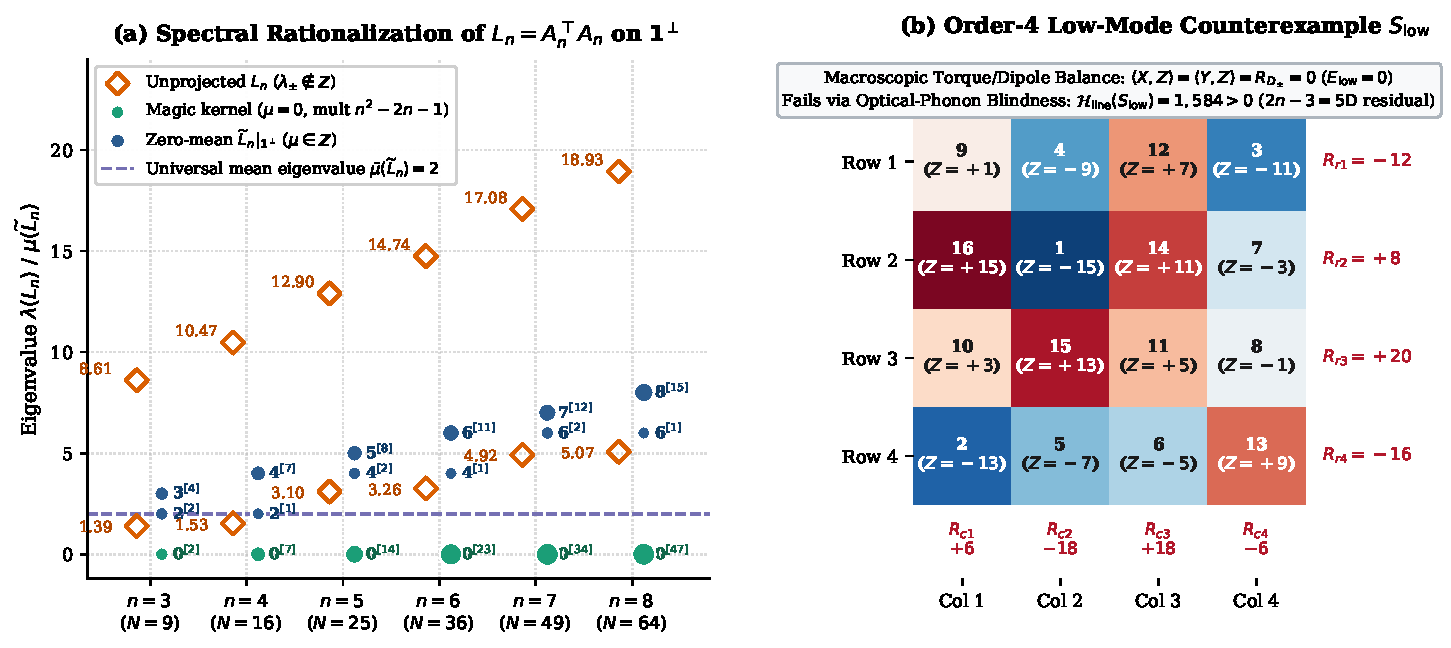
\includegraphics[width=\textwidth]{figures/fig1_spectral_operator.pdf}
  \caption{\textbf{Zero-mean spectrum of the line-incidence Laplacian $L_n = A_n^\top A_n$ and low-mode moment insufficiency.} \textbf{(a)} Comparison of the unprojected eigenvalues $\lambda(L_n)$ on $\R^{n^2}$ (hollow orange diamonds, showing the irrational branches $\lambda_\pm(n)$) against the zero-mean restricted spectrum $\mu(\Ltilde_n|_{\mathbf{1}^\perp})$ (filled navy and green circles, labeled $\mu^{[\mathrm{mult}]}$) for orders $n=3\dots 8$. Restricting to $\mathbf{1}^\perp$ yields integer eigenvalues with mean $\bar{\mu}(\Ltilde_n) = 2$ (dashed purple line). \textbf{(b)} Explicit $4\times 4$ counterexample $S_{\mathrm{low}}$ (\Cref{rem:low_mode_insufficiency}) whose linear dipole moments $\langle X,Z\rangle = \langle Y,Z\rangle = 0$ and main diagonals $R_{D_\pm} = 0$ vanish ($E_{\mathrm{low}}=0$), yet whose quadratic and cubic row/column moments produce $\Hline(S_{\mathrm{low}}) = 1{,}584 > 0$.}
  \label{fig:spectral}
\end{figure}

\begin{table}[t]
\centering
\caption{Spectral invariants of the unprojected operator $L_n$ on $\R^{n^2}$ and zero-mean operator $\Ltilde_n$ on $\mathbf{1}^\perp$ across orders $n=3\dots 8$, verified by \texttt{verify\_paper\_d.py}.}
\label{tab:spectral_census}
\footnotesize
\setlength{\tabcolsep}{4pt}
\begin{tabular}{@{}cccccccc@{}}
\toprule
$n$ & $N=n^2$ & $\operatorname{rank}(A_n)$ & $\dim\ker(L_n)$ & Irrational $\lambda_\pm(L_n)$ & Zero-Mean $\spec(\Ltilde_n|_{\mathbf{1}^\perp})$ & $\tr(\Ltilde_n)$ & $\mathbb{E}[\Hline(S)] = 2\|\mathbf{z}\|^2$ \\
\midrule
$3$ & $9$  & $7$  & $2$  & $1.3944,\; 8.6056$ & $\{0^{[2]}, 2^{[2]}, 3^{[4]}\}$ & $16$  & $480$ \\
$4$ & $16$ & $9$  & $7$  & $1.5279,\; 10.4721$ & $\{0^{[7]}, 2^{[1]}, 4^{[7]}\}$ & $30$  & $2{,}720$ \\
$5$ & $25$ & $11$ & $14$ & $3.1010,\; 12.8990$ & $\{0^{[14]}, 4^{[2]}, 5^{[8]}\}$ & $48$  & $10{,}400$ \\
$6$ & $36$ & $13$ & $23$ & $3.2554,\; 14.7446$ & $\{0^{[23]}, 4^{[1]}, 6^{[11]}\}$ & $70$  & $31{,}080$ \\
$7$ & $49$ & $15$ & $34$ & $4.9172,\; 17.0828$ & $\{0^{[34]}, 6^{[2]}, 7^{[12]}\}$ & $96$  & $78{,}400$ \\
$8$ & $64$ & $17$ & $47$ & $5.0718,\; 18.9282$ & $\{0^{[47]}, 6^{[1]}, 8^{[15]}\}$ & $126$ & $174{,}720$ \\
\bottomrule
\end{tabular}
\end{table}

\subsection{Insufficiency of Linear Dipole Moments and the \texorpdfstring{$(2n-4)$}{(2n-4)}-Dimensional Higher-Degree Moment Subspace}

In Paper~II \cite{mathewson2026moments} and Paper~III \cite{mathewson2026mechanics}, we proved that semi-magic row and column balance implies vanishing linear dipole moments $\langle X,Z\rangle = \langle Y,Z\rangle = 0$, so that every magic square has an isotropic inertia tensor. A natural question is whether the converse holds when supplemented by the two main diagonal constraints: if a permutation $S \in S_{n^2}$ satisfies zero dipole tilt ($\langle X,Z\rangle = \langle Y,Z\rangle = 0$) and zero diagonal residuals ($R_{D_+} = R_{D_-} = 0$), must $S$ be a magic square? By \Cref{prop:spectral_rationalization}, the answer is negative for all $n \ge 3$:

\begin{remark}[Insufficiency of Linear Dipole and Diagonal Moments]
\label{rem:low_mode_insufficiency}
Define the $4$-mode dipole-plus-diagonal energy functional
\begin{equation}
  E_{\mathrm{low}}(S) = \langle X,Z\rangle^2 + \langle Y,Z\rangle^2 + R_{D_+}(S)^2 + R_{D_-}(S)^2.
  \label{eq:E_low_def}
\end{equation}
Because $X \in \mathcal{V}_{\mathrm{col}}$ and $Y \in \mathcal{V}_{\mathrm{row}}$ are linear (degree-$1$) column and row coordinate vectors, they are mutually orthogonal and orthogonal to the projected diagonal vectors $\widetilde{\mathbf{d}}_\pm \in \mathcal{V}_{\mathrm{row}}\otimes\mathcal{V}_{\mathrm{col}}$. Thus $\{X, Y, \widetilde{\mathbf{d}}_+, \widetilde{\mathbf{d}}_-\}$ spans a $4$-dimensional subspace of the $2n$-dimensional active zero-mean image $\operatorname{im}(\Ltilde_n) = \mathcal{V}_{\mathrm{row}} \oplus \mathcal{V}_{\mathrm{col}} \oplus \operatorname{span}\{\widetilde{\mathbf{s}}_d, \mathbf{a}_d\} \subset \mathbf{1}^\perp$. Its orthogonal complement inside $\operatorname{im}(\Ltilde_n)$ has dimension
\begin{equation}
  \dim\bigl(\operatorname{im}(\Ltilde_n) \cap \ker(E_{\mathrm{low}})\bigr) = 2n - 4 = 2(n-2),
  \label{eq:high_mode_dim}
\end{equation}
spanned by the $n-2$ higher-degree orthogonalized column polynomial moments $P_k(X) \in \mathcal{V}_{\mathrm{col}}$ and $n-2$ row polynomial moments $P_k(Y) \in \mathcal{V}_{\mathrm{row}}$ of degrees $2 \le k \le n-1$, all of which share the flat eigenvalue $\mu = n$ under $\Ltilde_n$. At order $n=4$ ($2n-4 = 4$ unconstrained polynomial modes corresponding to $\langle X^2,Z\rangle, \langle X^3,Z\rangle, \langle Y^2,Z\rangle, \langle Y^3,Z\rangle$), the explicit permutation
\begin{equation}
  S_{\mathrm{low}} = \begin{bmatrix}
    9 & 4 & 12 & 3 \\
    16 & 1 & 14 & 7 \\
    10 & 15 & 11 & 8 \\
    2 & 5 & 6 & 13
  \end{bmatrix} \in S_{16}
  \label{eq:S_low_matrix}
\end{equation}
satisfies $\langle X,Z\rangle = 0$, $\langle Y,Z\rangle = 0$, $R_{D_+}(S_{\mathrm{low}}) = 0$, and $R_{D_-}(S_{\mathrm{low}}) = 0$ ($E_{\mathrm{low}}(S_{\mathrm{low}}) = 0$), yet exhibits non-zero row residuals $\mathbf{R}_{\mathrm{row}} = (-12, +8, +20, -16)$, column residuals $\mathbf{R}_{\mathrm{col}} = (+6, -18, +18, -6)$, and total line energy $\Hline(S_{\mathrm{low}}) = 1{,}584 > 0$ (\Cref{fig:spectral}b).
\end{remark}

\Cref{rem:low_mode_insufficiency} explains why macroscopic rigid-body torque and moment-of-inertia balance cannot synthesize magic squares on their own: any physical relaxation that couples only to global center-of-mass tilt ($\langle X,Z\rangle, \langle Y,Z\rangle$) and principal diagonal sums ($R_{D_\pm}$) constrains only $4$ linear directions in $\mathbf{1}^\perp$ and is blind to the $2n-4$ higher-degree polynomial row and column moments ($\langle X^k,Z\rangle, \langle Y^k,Z\rangle$ for $2 \le k \le n-1$). At the same time, \Cref{prop:spectral_rationalization} defines the \emph{nullspace-to-constraint ratio} on the zero-mean hyperplane $\mathbf{1}^\perp$:
\begin{equation}
  \eta_{\mathrm{MC}}(n) = \frac{\dim\ker(\Ltilde_n)}{\operatorname{rank}(\Ltilde_n)} = \frac{n^2 - 2n - 1}{2n},
  \label{eq:maxwell_calladine_ratio}
\end{equation}
analogous to the ratio of internal zero-energy degrees of freedom to active linear constraints in Maxwell--Calladine constraint counting \cite{maxwell1864calculation,calladine1978buckminster}. Note an important distinction between continuous and discrete settings: in continuous linear algebra on $\mathbf{1}^\perp$, $\dim\ker(\Ltilde_n) = n^2-2n-1 > 0$ for every $n \ge 3$, so the linear system $A_n\mathbf{z} = \mathbf{0}$ always possesses a non-trivial nullspace. What makes small orders $n \in \{3,4,5\}$ combinatorially frustrated is the \emph{discrete permutation constraint} $\mathbf{z} \in S_{n^2}$---that is, finding vertices of the permutahedron that lie inside $\ker(\Ltilde_n)$ when $\dim\ker(\Ltilde_n)$ is smaller than or comparable to the rank $2n$ ($\eta_{\mathrm{MC}}(3) = 0.33$, $\eta_{\mathrm{MC}}(4) = 0.88$, $\eta_{\mathrm{MC}}(5) = 1.40$). As $n \ge 6$ grows, the nullspace dimension expands quadratically while the constraint rank grows only linearly ($\eta_{\mathrm{MC}}(8) = 2.94$, $\eta_{\mathrm{MC}}(10) = 3.95$), producing the discrete dimensional relief quantified in \Cref{sec:bubble}.
